\documentclass[a4paper]{article}

\usepackage[spanish]{babel}
\usepackage{graphicx}
\usepackage{amsmath, amssymb}
\usepackage[margin=2cm]{geometry}
\usepackage{fancyhdr}
\usepackage{enumerate}
\usepackage[shortlabels]{enumitem}
\usepackage{parskip}
\usepackage[most]{tcolorbox}
\usepackage[hidelinks]{hyperref}
\usepackage{float}


% cabecera
\pagestyle{fancy}
\fancyhead[l]{Daniel Soto}
\fancyhead[c]{Problemas de Astronomía \#9}
\fancyhead[r]{\today}
\fancyfoot[c]{\thepage}
\renewcommand{\headrulewidth}{0.2pt} % linea horizontal

%% Definicion de comandos para formato de unidades fisicas %%
\newcommand{\m}{\text{m}}
\newcommand{\cm}{\text{cm}}
\newcommand{\km}{\text{km}}
\newcommand{\s}{\text{s}}
\newcommand{\N}{\text{N}}
\newcommand{\g}{\text{g}}
\newcommand{\kg}{\text{kg}}
\newcommand{\Msolar}{\text{M}_\odot}
\newcommand{\Mterrestre}{\text{\text{M}_\oplus}}
\newcommand{\AU}{\text{AU}}
\newcommand{\ly}{\text{ly}}
\newcommand{\nT}{\text{nT}}
\newcommand{\GeV}{\text{GeV}}
\newcommand{\atomscm}{\text{atoms/cm}^3}
\newcommand{\K}{\text{K}}
\newcommand{\J}{\text{J}}



\newcounter{problema}

\newtcolorbox[use counter=problema]{problema}[1][]{%
	breakable,
    colback=gray!15,
    colframe=gray!60,
    fonttitle=\bfseries,
    title={Problema~\theproblema:},
    boxrule=0.5mm,
    arc=3mm,
    boxsep=5pt,
    left=8pt,
    right=8pt,
    top=6pt,
    bottom=6pt,
    #1
}


\begin{document}

\begin{problema}
\textbf{Funciones Monstruosas en Ciencia Espacial I}:  Olvida las fórmulas sencillas con las que has jugado antes. Aquí tienes una fórmula razonablemente compleja que tendrás que evaluar, y que involucrará todas las habilidades que has aprendido previamente en álgebra... ¡y también un dominio de la notación científica!

\begin{figure}[H]
        \centering
        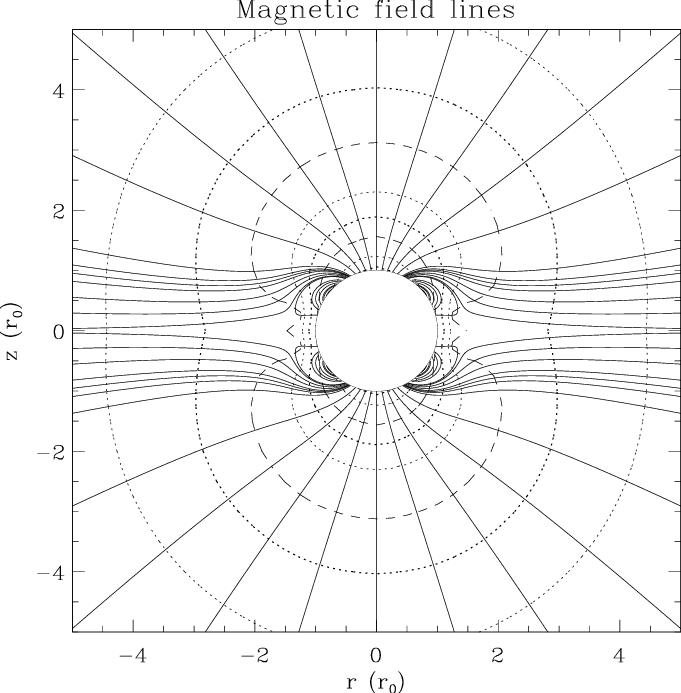
\includegraphics[width=0.6\textwidth]{MagneticField.png}
        \caption{Banaszkiewicz, M., Axford, W., \& McKenzie, J. (1998). An analytic solar magnetic field model. Astronomy and Astrophysics, 337, 940–944.}
        \label{fig:1}
    \end{figure}
    
\begin{equation}
\frac{B_\rho}{M}=\frac{3\rho z}{r^5} + \frac{15Q}{8}\frac{\rho z}{r^7}\frac{\left(4z^2-3\rho^2\right)}{r^2} +
 \frac{K}{a_1} \frac{\rho}{\left[(|z|+a_1)^2 + \rho^2\right]^{3/2}}
\label{eq:1}
\end{equation}

\begin{equation}
\frac{B_z}{M} = \frac{2z^2-\rho^2}{r^5} + \frac{3Q}{8}\frac{\left(8z^4+3\rho^4-24\rho^2 z^2\right)}{r^9} + 
\frac{K}{a_1} \frac{|z|+a_1}{\left[(|z|+a_1)^2+\rho^2\right]^{3/2}}
\label{eq:2}
\end{equation}

Estas fórmulas dan las dos componentes del campo magnético solar, en unidades de Gauss, donde $B = B_\rho \rho + B_z z$, siendo $\rho$ y $z$ los vectores unitarios a lo largo de estas dos direcciones.

\begin{enumerate}
	\item Evalúa las componentes $B_\rho$ y $B_z$ para las siguientes condiciones, apropiadas para una distancia desde el Sol igual a la órbita de la Tierra, utilizando la siguiente información:

    $$r^2 = \rho^2+z^2\quad$$
    
    donde
    \begin{itemize}
	\item $M = 6.03 \times 10^{17} \km^3$
    	\item$a_1 = 1.07 \times 10^{6}\km$
	\item $K=1$
   	\item $Q = 1.5$
    	\item $z = -3.48 \times 10^{7} \km$
    	\item $\rho = 1.46 x 10^8 \km$
   \end{itemize}
    
	\item Encuentra la magnitud del campo magnético utilizando los valores de las dos componentes calculadas en el item 1.

	\item  Explica qué efecto tiene $|z|$ en la representación gráfica del campo magnético.
\end{enumerate}
\end{problema}
[9] \cite{NASA_SpaceMathIII}

\bibliographystyle{plainurl}
\bibliography{bibliografia} % Nombre del .bib

\end{document}
